\documentclass[10pt,a4paper,titlepage]{report}
\usepackage[utf8]{inputenc}
\usepackage[spanish,es-tabla]{babel}
\usepackage{amsmath}
\usepackage{amsfonts}
\usepackage{amssymb}
\usepackage{float}
\usepackage{graphicx}
\usepackage{abstract}
\usepackage{caption}
%\captionsetup[table]{name=Tabla}

\usepackage{subcaption}
\usepackage{listings}

%\usepackage{listingsutf8}
\usepackage{xcolor}
\usepackage{pdfpages} %para abrir documentos en PDF
\usepackage{xr} %Para referenciar etiquetas desde otros ficheros
\usepackage{underscore} %Para que lea bien el código
\usepackage{hyperref}% Para que el índice tenga hipervínculos
\usepackage[left=2cm,right=2cm,top=2cm,bottom=2cm]{geometry}
\lstdefinestyle{customc}{
  belowcaptionskip=1\baselineskip,
  breaklines=true,
  frame=L,
  xleftmargin=\parindent,
  language=C,
  showstringspaces=false,
  basicstyle=\footnotesize\ttfamily,
  keywordstyle=\bfseries\color{green!40!black},
  commentstyle=\itshape\color{purple!40!black},
  identifierstyle=\color{blue},
  stringstyle=\color{orange},
}

\lstset{style=customc,literate=
  {á}{{\'a}}1 {é}{{\'e}}1 {í}{{\'i}}1 {ó}{{\'o}}1 {ú}{{\'u}}1
  {Á}{{\'A}}1 {É}{{\'E}}1 {Í}{{\'I}}1 {Ó}{{\'O}}1 {Ú}{{\'U}}1
  {à}{{\`a}}1 {è}{{\`e}}1 {ì}{{\`i}}1 {ò}{{\`o}}1 {ù}{{\`u}}1
  {À}{{\`A}}1 {È}{{\'E}}1 {Ì}{{\`I}}1 {Ò}{{\`O}}1 {Ù}{{\`U}}1
  {ä}{{\"a}}1 {ë}{{\"e}}1 {ï}{{\"i}}1 {ö}{{\"o}}1 {ü}{{\"u}}1
  {Ä}{{\"A}}1 {Ë}{{\"E}}1 {Ï}{{\"I}}1 {Ö}{{\"O}}1 {Ü}{{\"U}}1
  {â}{{\^a}}1 {ê}{{\^e}}1 {î}{{\^i}}1 {ô}{{\^o}}1 {û}{{\^u}}1
  {Â}{{\^A}}1 {Ê}{{\^E}}1 {Î}{{\^I}}1 {Ô}{{\^O}}1 {Û}{{\^U}}1
  {ã}{{\~a}}1 {ẽ}{{\~e}}1 {ĩ}{{\~i}}1 {õ}{{\~o}}1 {ũ}{{\~u}}1
  {Ã}{{\~A}}1 {Ẽ}{{\~E}}1 {Ĩ}{{\~I}}1 {Õ}{{\~O}}1 {Ũ}{{\~U}}1
  {œ}{{\oe}}1 {Œ}{{\OE}}1 {æ}{{\ae}}1 {Æ}{{\AE}}1 {ß}{{\ss}}1
  {ű}{{\H{u}}}1 {Ű}{{\H{U}}}1 {ő}{{\H{o}}}1 {Ő}{{\H{O}}}1
  {ç}{{\c c}}1 {Ç}{{\c C}}1 {ø}{{\o}}1 {å}{{\r a}}1 {Å}{{\r A}}1
  {€}{{\euro}}1 {£}{{\pounds}}1 {«}{{\guillemotleft}}1
  {»}{{\guillemotright}}1 {ñ}{{\~n}}1 {Ñ}{{\~N}}1 {¿}{{?`}}1 {¡}{{!`}}1 }

\title{
\includegraphics[width=0.75\textwidth]{../OdiTech Logo.pdf}  \\
\vspace*{1in}
\textbf{Informe Técnico - Económico}\\
\vspace*{0.5in}
\textbf{Taller de Proyectos II}}

\author{Autores:\\
Inés Varona Peña, David Manso Fernández, Óscar Martín Casares y Daniel Sirgo Rodríguez\\
		\vspace*{0.5in} \\
        \textbf{Universidad de Valladolid}\\
        Valladolid, España
       } \date{\today}

\begin{document}
\maketitle
\tableofcontents
\listoffigures
\listoftables

\chapter{Introducción}
	
La empresa para la que trabajamos ha sido adjudicataria de un contrato con el objetivo de desarrollar un servicio de vehículo conectado consistente en el envío de información de vídeo desde el vehículo a un servidor en el \textit{Cloud}. El vídeo será procesado en \textit{Cloud} para la detección automática, mediante técnicas de inteligencia artificial, de señales de tráfico en la carretera.\\

El objetivo de este proyecto es desarrollar una infraestructura de red 4G que permita la transmisión de vídeo desde los vehículos conectados al servidor \textit{Cloud}. Esta infraestructura permitirá a la empresa ofrecer un servicio de predicción de señales de tráfico en la carretera, lo que ayudará a mejorar la seguridad y la eficiencia en el tráfico. Esto se logrará desarrollando un demostrador previo al despliegue de la red para probar la capacidad de la empresa para desplegar el servicio, y presentando una memoria técnico-económica que detalle el despliegue de la red en el tramo de autovía A-62 desde el kilómetro 158 hasta el kilómetro 231. Además, la empresa tendrá que demostrar contar con los permisos legales pertinentes para el despliegue del servicio, que tendrá una duración máxima de 6 meses.

Los componentes que la empresa pone a nuestra disposición son herramientas esenciales para el desarrollo de proyectos en infraestructura de telecomunicaciones y en inteligencia artificial.\\

En primer lugar, contamos con ordenadores de sobremesa y memorias USB, que nos permiten trabajar en el desarrollo de algoritmos de inteligencia artificial y en la programación de los módems Huawei y las tarjetas SIM de Vodafone S.A.U. para la emulación de la red 4G.\\

Asimismo, disponemos de un sistema SDR (\textit{Software Defined Radio}) BladeRF 2.0 xa9, un dispositivo que permite la recepción y transmisión de señales de radio en un amplio rango de frecuencias. Este sistema se controla mediante el \textit{software} abierto srsRAN, que nos permite configurar y gestionar las comunicaciones.\\

En cuanto a las frecuencias, se usan las de banda 7. En concreto el rango que va de 2540 a 2550 MHz y de 2650 a 2670 MHz. Estas frecuencias se utilizan para probar y validar el funcionamiento de las comunicaciones.\\

Para emular la transmisión de vídeo, la empresa nos proporciona vehículos Azon DeepRacer Evo dirigidos por control remoto, junto con la información básica de su manejo. Estos vehículos nos permiten simular las condiciones reales de transmisión de vídeo en diferentes entornos.\\

Además, contamos con un conjunto modular de pistas y señales que nos permiten montar diversos circuitos para probar y validar diferentes escenarios de comunicación.\\

Por último, la empresa nos proporciona bibliotecas Python para aprendizaje automático y recursos de computación en la nube para ejecutar los algoritmos de aprendizaje automático. Estas herramientas nos permiten desarrollar y probar modelos de inteligencia artificial para mejorar la eficiencia y la seguridad de las comunicaciones.

\chapter{Planteamiento inicial}
	Partimos de la base de que somos una empresa a la que se la ha adjudicado el despliegue de infraestructura de red 4G, con el objetivo de prestar servicio a vehículos conectados. Dicho servicio queremos que se implemente en la autovía que conecta la ciudad de Salamanca con Tordesillas, en Castilla y León. \\

El tramo de carretera seleccionado comprende 73 kilómetros, en concreto desde el kilómetro 158 al kilómetro 231 de la A-62. En dicho tramo nos encontramos con que ya existe una buena infraestructura de red 4G prestando servicio, por ello vamos a aprovechar parte de ella. En concreto, haremos uso de las torres de telefonía ya disponibles, disponemos de 11 a lo largo de la carretera, tal y como podemos observar en la figura \ref{autovia}. En las torres que sean necesarias (que no tienen por qué ser todas) instalaremos nuestros propios equipos, como estaciones base y antenas. Es importante evaluar cuidadosamente los costes asociados a los componentes y considerar opciones con precios competitivos. \\


\begin{figure}[H]
    \centering
 	\includegraphics[width=\textwidth]{Imagenes/PlanteamientoInicial/torres_telefonia.pdf}
    \caption{Mapa de la autovía A-62 y las torres de comunicación existentes }
    \label{autovia}
\end{figure}

Queremos que un número elevado de coches pueda hacer uso de dicho servicio de manera ininterrumpida, es decir, que cada coche tenga capacidad suficiente para enviar el vídeo captado por la cámara durante todo el recorrido. Por eso, es necesario disponer de un ancho de banda de al menos varios Mbps, todo dependiendo de la calidad del vídeo que queramos ofrecer. \\

Prestando este servicio, los vehículos de los usuarios tendrán la capacidad de detectar las señales de tráfico aumentando así la seguridad vial, ya que así los vehículos pueden adaptar su velocidad y comportamiento en la carretera, lo que puede reducir el riesgo de accidentes y mejorar la seguridad en general. De igual forma, puede fomentar el cumplimiento de las normativas y regulaciones de tráfico, disminuir la cantidad de sanciones, o puede ayudar a optimizar el consumo de combustible y moderar las emisiones de gases contaminantes procedentes de dichos vehículos.\\

La seguridad en las carreteras es uno de los temas más importantes en el mundo actual. Una de las medidas para garantizar la seguridad es la señalización vial, la cual indica a los conductores las condiciones y normas de circulación. Sin embargo, a menudo las señales pueden ser difíciles de identificar debido a factores como su ubicación, desconocimiento de la misma o la distracción del conductor.\\

Para resolver este problema, se puede utilizar el aprendizaje automático para diseñar modelos capaces de detectar de manera precisa y eficiente las señales de tráfico. Estos modelos pueden ayudar a mejorar la seguridad en las carreteras al permitir que los conductores reciban información clara y precisa en todo momento.\\

En este contexto, nuestra empresa ha sido encargada de diseñar e implementar un modelo de aprendizaje automático para la detección de señales de tráfico. Para eso, debemos utilizar técnicas avanzadas de procesamiento de imágenes. El objetivo final es contribuir a la seguridad en las carreteras y ofrecer soluciones innovadoras y eficaces.\\

Con el objetivo de poder prestar dicho servicio, se debe elegir qué modelo de inteligencia artificial se va a seleccionar para llevarlo a cabo. En el campo de la detección de objetos en imágenes y vídeos, existen varios modelos de aprendizaje automático que se pueden utilizar. Uno de los más avanzados y precisos es YOLO. Lo que le distingue de otros modelos es su capacidad para detectar múltiples objetos en una sola imagen de manera eficiente y precisa, utilizando redes neuronales convolucionales (CNN) y técnicas de filtrado de cajas delimitadoras. \\



\chapter{Solución}
	\section{Infraestructura}
		En primera instancia, se debe decidir cómo se quiere plantear la infraestructura de red, si vamos a construir nuestras propias torres o no, si vamos a funcionar como una operadora virtual o si por el contrario vamos a comprar a instalar nuestros propios equipos. En nuestro caso, nos hemos decantado por alquilar las torres de telecomunicaciones existentes, en la cuales vamos a instalar nuestros propios componentes. De esta manera, lograremos diseñar una red que cumple con compromisos económicos y que a la vez nos proporcionan cierto control en caso de averías o problemas.\\

Luego, debemos conocer dónde se encuentran las torres de telecomunicaciones existentes. Existen varias páginas web a través de las cuales podemos conocer dicha información, como Infoantenas \url{https://geoportal.minetur.gob.es/VCTEL/vcne.do}, un servicio desarrollado por parte del Ministerio de Asuntos Económicos y Transformación Digital, o AntenasGSM \url{https://antenasgsm.com}. A través de dichas páginas hemos podido conocer la localización de las torres, mostradas en la figura \ref{autovia}.\\

Sin embargo, tras seleccionar el modelo de estación base y antena que vamos a utilizar, en función de sus distintas características técnicas hemos propuesto un diseño de infraestructura, en la cual no va a ser necesario utilizar todas las torres de telecomunicaciones disponibles. Existen 11 torres desplegadas y utilizaremos 7 de ellas. En origen las distintas torres pertenecían a las propias empresas operadoras que prestan el propio servicio, o empresas filiales de las mísmas. No obstante, la mayoría de ellas han vendido una gran cantidad de las torres a otras empresas, como pueden ser Cellnex Telecom, una empresa española, o American Tower Corporation, empresa estadounidense, ambas se dedican a la construcción y gestión de infraestructuras de telecomunicaciones. [Ref: Telefónica vende a ATC las torres de Telxius por 7.700 millones de euros | Empresas (elmundo.es) y Orange vende 1.500 torres a Cellnex para usarlas en régimen de alquiler | Empresas (elmundo.es)]. Se estima que el alquiler de estas torres se encuentra en torno a los 4.000 y 20.000 euros en zonas urbanas, y 1.000 y 15.000 euros en zonas rurales, costo que habrá que tener en cuenta a la hora de presupuestar la infraestructura.\\

Para el diseño del proyecto se ha contactado con los principales distribuidores en España de estos componentes, como pueden ser Ericsson, Nokia, Kathrein o Moyano Telsa, con el objetivo de lograr una red lo más similar a lo que nos podemos encontrar en las grandes operadoras españolas. Sin embargo, ninguna de estas empresas nos ha respondido ni nos has facilitado un catálogo de sus productos, por ello, hemos procedido a diseñar la red con equipos de los cuales si hemos podido encontrar información. \\

En primer lugar, hemos seleccionado una estación base proporcionada por una empresa china llamada Baicells, una compañía fundada en 2014 con sede en cinco continentes que ofrece productos de tecnología inalámbrica 4G y 5G. El modelo concreto es el Nova846, éste nos proporcionará una potencia de transmisión entre 0 y 37 dBm, una distancia máxima de 60km y una sensibilidad diferente en función del rango de distancias en el que se encuentra el usuario gracias a la modulación adaptativa.\\

\begin{table}[H]
\centering
\begin{tabular}{|c|c|c|}
\hline
\textbf{Esquema de modulación} & \textbf{RSRP {[}dBm{]}}            & \textbf{Distancia cubierta {[}km{]}} \\ \hline \hline
QPSK                           & -120 \textless RSRP \textless -110 & Entre 40 y 60                        \\ \hline
16 QAM                         & -110 \textless RSRP \textless -100 & Entre 10 y 40                        \\ \hline
64 QAM                         & -100 \textless RSRP \textless -85  & Entre 4 y 10                         \\ \hline
256 QAM                        & RSRP \textgreater -85              & Menor a 4                            \\ \hline
\end{tabular}
\caption{Cobertura en función de la modulación.}
\label{cobertura}
\end{table}

Dependiendo de la configuración proporcionará un rendimiento u otro, en nuestro caso nos hemos decidido por la configuración 6. Ésta nos brindará un rendimiento máximo en el enlace de subida, que nos interesa que sea máximo para que el mayor número de usuarios pueda enviar el vídeo en streaming. Lograremos tener las distintas capacidades mostradas para el enlace de downlink y uplink.\\

\begin{table}[H]
\centering
\begin{tabular}{|c||c|c|}
\hline
\textbf{Modulación} & \textit{\textbf{DownLink}} & \textit{\textbf{UpLink}} \\ \hline \hline
256 QAM             & 348 Mbps                   & 92 Mbps                  \\ \hline
64 QAM              & 264 Mbps                   & 70 Mbps                  \\ \hline
16 QAM              & 70 Mbps                    & 53 Mbps                  \\ \hline
QPSK                & 53 Mbps                    & 53 Mbps                  \\ \hline
\end{tabular}
\caption{Capacidades del enlace de bajada y de subida}
\label{capacidad}
\end{table}

La antena seleccionada es fabricada por la empresa irlandesa Alpha Wireless, una compañía fundada en 2006 dedicada a la fabricación de antenas. El modelo seleccionado es el AW3864-E-F, una antena sectorial de 4G que nos proporciona un ancho de haz de 65$\deg$ y una ganancia de 18 dB en las frecuencias de interés.\\

Con estos datos nos encontramos en disposición de simular la infraestructura, para ello hemos utilizado la herramienta de planificación y diseño de redes de telecomunicaciones Xirio-online. Una plataforma desarrollada una empresa española llamada Xirio, especializada en soluciones de ingeniería para telecomunicaciones. Con ésta se pueden crear mapas de cobertura y realizar simulaciones de propagación de señal con redes de telefonía móvil o televisión digital entre otras, así como evaluar del rendimiento de la red.\\

A través de un estudio de multicobertura e introduciendo todos los parámetros ya mencionados en la herramienta, hemos dispuesto las antenas a lo largo de tramo de autovía en las distintas ubicaciones en las que previamente localizamos las torres de telecomunicaciones. Como se puede apreciar en la figura \ref{xirio} teniendo en cuenta la cartografía del terreno, podremos cubrir la carretera a través de 7 estaciones base y 12 antenas. Asimismo, dado que no hemos logrado averiguar la altura exacta de cada una de las torres utilizadas, hemos supuesto una altura de 30 metros para todas ellas, ya que la altura media se encuentre en 15 y 50 metros.

\begin{figure}[H]
\centering
\includegraphics[width=\textwidth]{Imagenes/Solucion/xirio.pdf}
\caption{Distribución de la cobertura y estudio de cobertura}
\label{xirio}
\end{figure}

Un detalle muy importante del proyecto es conocer cuál es la cantidad de usuarios a la que se podrá prestar el servicio de detección de señales de tráfico. Tal y como hemos distribuido las antenas y estaciones base, en prácticamente la totalidad de la autovía se proporciona una potencia suficiente como para que los usuarios operen a través de la modulación 256 QAM. De este modo, podremos calcular la cantidad de usuarios a la cual podremos prestar servicio en función de las distintas velocidades que nos podríamos encontrar.  Dividiendo la capacidad del enlace de subida entre la cantidad de Mbps necesarios para transmitir por cada usuario, podremos conocer el número de usuarios posible de manera simultánea, teniendo en cuenta además cuál es la distancia y fotogramas por segundo adecuados para poder detectar la señal con fiabilidad.

\begin{table}[H]
\centering
\begin{tabular}{|c|c|c|c|c|}
\hline
\textbf{Distancia} & \textbf{Velocidad} & \textbf{Frames/Sec} & \textbf{Mbps} & \textbf{Cantidad Usuarios} \\ \hline \hline
20 metros          & 80 km/h            & 12 f/s              & 2 Mbps        & 46 usuarios                \\ \hline
20 metros          & 100 km/h           & 15 f/s              & 2,5 Mbps      & 36 usuarios                \\ \hline
20 metros          & 120 km/h           & 18 f/s              & 3 Mbps        & 30 usuarios                \\ \hline
\end{tabular}
\caption{Cantidad de usuarios disponibles en función de la velocidad del vehículo }
\label{users}
\end{table}

La interconexión entre las estaciones base y el núcleo de la red 4G se establecerá utilizando una topología de estrella, donde el núcleo se situará en Madrid junto con el centro de operaciones (CTO). Esta elección permite centralizar la gestión completa del servicio en una ubicación, lo que brinda ventajas logísticas en caso de necesitar intervenciones. La elección de Madrid se basa en su ubicación geográfica estratégica y en la disponibilidad de abundantes recursos.\\

El core de la red 4G, esencial para proporcionar servicios de conectividad y gestionar el tráfico de datos, se implementará utilizando la solución Telrad BreezeWAY2020 de Telrad Networks. Telrad Networks, una empresa líder en el sector de las telecomunicaciones desde 1951, ofrece esta solución que tiene la capacidad de atender simultáneamente a 10.000 usuarios. Además, cuenta con una Arquitectura de Clúster Distribuido que permite un escalado gradual y prácticamente ilimitado en términos de capacidad y rendimiento a nivel de red.\\

El centro de operaciones se encargará de la detección de señales de tráfico utilizando modelos de inteligencia artificial, como YOLO v3. Dado el alto requerimiento computacional de este servicio, ha surgido el debate sobre si es más conveniente adquirir una gran cantidad de servidores o bien optar por servicios en la nube ofrecidos por grandes empresas tecnológicas como AWS (Amazon) o Azure (Microsoft).\\

En el contexto de los vehículos autónomos, se ha observado una tendencia creciente hacia la realización del cálculo computacional en el propio vehículo. Esto se debe a que delegar un mayor acceso y control externo aumenta los riesgos de seguridad. Por lo tanto, resulta más seguro realizar el procesamiento de datos en el vehículo mismo.\\

En línea con esta consideración, se ha decidido alquilar los servicios de AWS, ya que una inversión inicial significativa no sería viable a largo plazo, dado que en el futuro estos servicios podrían no utilizarse para este propósito.\\

El núcleo de nuestra red establece su conectividad a Internet mediante un enlace de conexión dedicado, el cual puede ser suministrado por un proveedor de servicios de Internet (ISP) o a través de una conexión de fibra óptica. Es fundamental que este enlace posea una velocidad y fiabilidad adecuadas para gestionar eficientemente el tráfico de datos generado por los usuarios de la red 4G.

		
	\section{Detección de señales de tráfico}
		La seguridad en las carreteras es uno de los temas más importantes en el mundo actual. Una de las medidas para garantizar la seguridad es la señalización vial, la cual indica a los conductores las condiciones y normas de circulación. Sin embargo, a menudo las señales pueden ser difíciles de identificar debido a factores como su ubicación, desconocimiento de la misma o la distracción del conductor.\\

Para resolver este problema, se puede utilizar el aprendizaje automático para diseñar modelos capaces de detectar de manera precisa y eficiente las señales de tráfico. Estos modelos pueden ayudar a mejorar la seguridad en las carreteras permitiendo que los conductores reciban información clara y precisa en todo momento.\\

En este contexto, nuestra empresa ha sido encargada de diseñar e implementar un modelo de aprendizaje automático para la detección de señales de tráfico. Para eso, debemos utilizar técnicas avanzadas de procesamiento de imágenes. El objetivo final es contribuir a la seguridad en las carreteras y ofrecer soluciones innovadoras y eficaces.\\

Con el objetivo de poder prestar dicho servicio, se debe elegir qué modelo de inteligencia artificial se va a seleccionar para llevarlo a cabo. En el campo de la detección de objetos en imágenes y vídeos, existen varios modelos de aprendizaje automático que se pueden utilizar. Uno de los más avanzados y precisos es YOLO. Lo que le distingue de otros modelos es su capacidad para detectar múltiples objetos en una sola imagen de manera eficiente y precisa, utilizando redes neuronales convolucionales (CNN) y técnicas de filtrado de cajas delimitadoras. \\

YOLO significa \textit{You Only Look Onc}e\  \url{https://pjreddie.com/darknet/yolo/}. Se le puso ese nombre debido a que la red neuronal solo se aplica una vez a la imagen completa, lo que permite una detección rápida y precisa de objetos. Una de las ventajas clave de YOLO es que puede detectar múltiples objetos en una sola imagen, prediciendo las etiquetas de clase y las ubicaciones de los objetos al mismo tiempo. La red neuronal divide la imagen en regiones, predice cajas delimitadoras o \textit{bounding boxes} y probabilidades para cada una de ellas, y filtra las cajas delimitadoras con una técnica llamada supresión no máxima para eliminar aquellas con baja confianza o superpuestas con otras de mayor confianza \cite{yolo1}.\\

El origen de YOLO se remonta al año 2015, fue desarrollado por Joseph Redmon, Santosh Divvala, Ross Girshick y Ali Farhadi mientras trabajaban en la Universidad de Washington. La primera versión de YOLO se presentó en un artículo titulado \textit{You Only Look Once: Unified, Real-Time Object Detection} en la conferencia de visión por ordenador CVPR (Computer Vision and Pattern Recognition) en 2016. \\

El éxito de YOLO se debió en gran parte a su capacidad para detectar objetos en tiempo real, con una velocidad de procesamiento mucho más rápida que otros algoritmos. Además, su precisión en la detección de objetos en imágenes fue muy alta en comparación en comparación con otros.\\

En 2016, Joseph Redmon fundó una empresa llamada "YOLO: You Only Look Once Inc." para desarrollar la tecnología de detección de objetos YOLO en un producto comercial. Sin embargo, en 2018, Redmon anunció que se retiraba de la investigación en inteligencia artificial debido a sus preocupaciones éticas sobre el uso de la tecnología de IA en aplicaciones militares.\\

A partir de entonces, la investigación y el desarrollo de YOLO fueron continuados por otros investigadores. Actualmente, hay cuatro versiones oficiales de YOLO: YOLOv1, YOLOv2, YOLOv3 y YOLOv4, donde cada versión ha mejorado en términos de precisión y velocidad de procesamiento, y ha incorporado nuevas técnicas de detección de objetos, como la eliminación de falsos positivos \cite{yolo2}.\\

En concreto, nosotros vamos a utilizar YOLO versión 3, la cual utiliza 53 capas convolucionales sucesivas. Seleccionamos esta versión ya que, debido al auge de estas tecnologías, quizás sea la versión con mayor documentación y ejemplos de los cuales aprender.\\

Lo normal cuando un particular se plantea desarrollar un proyecto de este tipo es trabajar a través de Google Colab o mediante sus propios recursos locales. Google Colab es una herramienta en línea que permite escribir, ejecutar y compartir código Python en un entorno de notebook en la nube con acceso a recursos \textit{hardware} de alta calidad y herramientas de desarrollo preinstaladas. Sin embargo, a pesar de que nuestros ordenadores no están especialmente pensados para trabajar con IA, decidimos utilizarlos frente a la plataforma de Google. Utilizando nuestros propios recursos optamos por premiar la sencillez y facilidad de trabajo frente a la alternativa de poseer un mejor \textit{hardware} online.\\

Dado que estamos hablando de software abierto, existen numerosas versiones de cada YOLO hechas por particulares. No obstante, la tercera versión oficial de YOLO se nutre de tres ficheros de configuración, el fichero de clases, el fichero que contiene la configuración de YOLO y el fichero que contiene los pesos resultados del entrenamiento del modelo.\\

Por defecto, viene pre-entrenado con el conjunto de datos COCO (\textit{Common Objects in Context}), que es un conjunto de datos de detección de objetos, que contiene más de 330.000 imágenes etiquetadas con más de 2,5 millones de instancias de objetos de 80 categorías diferentes, incluyendo personas, animales, vehículos, muebles y objetos de la vida cotidiana. Dicho pre-entrenamiento puede resultar muy útil para numerosas aplicaciones. Sin embargo, dado que nosotros queremos desplegar un sistema dedicado únicamente a la detección de señales de tráfico, trabajaremos con unos pesos especiales destinados a dicha operación.\\

El entrenamiento de algoritmos de detección de objetos puede ser muy costoso computacionalmente. El proceso de entrenamiento puede llevar varias horas, días o incluso semanas, dependiendo del tamaño del conjunto de datos y los recursos \textit{hardware} disponibles. Por ello, decidimos partir de pesos ya pre-entrenados en detección de señales.\\

Los pesos utilizados están preparados para detectar cuatro grupos de señales diferentes:\\
\begin{itemize}
\item Prohibición: señales circulares con fondo blanco y borde rojo, como puede ser una prohibición de superar una determinada velocidad o la prohibición de entrada de un vehículo en vía.
\item Peligro: señales triangulares con fondo blanco y borde rojo, como puede ser la señal de advertencia de una curva peligrosa o peligro de desprendimientos.
\item Obligación: señales circulares azules, como puede ser la obligación de superar determinada velocidad u obligación de realizar un giro.
\item Otros: resto de señales de tráfico.
\end{itemize}

Bajo estas premisas, mediante nuestra infraestructura de red 4G podemos poner en marcha el vehículo Amazon DeepRacer que tenemos en la figura \ref{deepracer}, así podremos manejar el vehículo y acceder al contenido de su cámara.\\

\begin{figure}[H]
    \centering
 	\includegraphics[width=0.6\textwidth]{Imagenes/IA/deepracer.pdf}
    \caption{Vehículo Amazon DeepRacer utilizado}
    \label{deepracer}
\end{figure}

Gracias a que nuestra escuela, ETSIT de la Universidad de Valladolid, poseía un pequeño circuito para trabajar con el vehículo, lo montamos y dispusimos varias señales de tráfico a lo largo de la maqueta. Así, pudimos probar el rendimiento de nuestro algoritmo de detección y los pesos de entrenamiento que posee. Tal y como podemos observar en las figuras \ref{deteccion1} y \ref{deteccion2}, logramos la detección de las señales a lo largo de la maqueta, a pesar de la calidad del vídeo y de que las señales miniatura no sean exactamente igual a las reales. \\

\begin{figure}[H]
    \centering
 	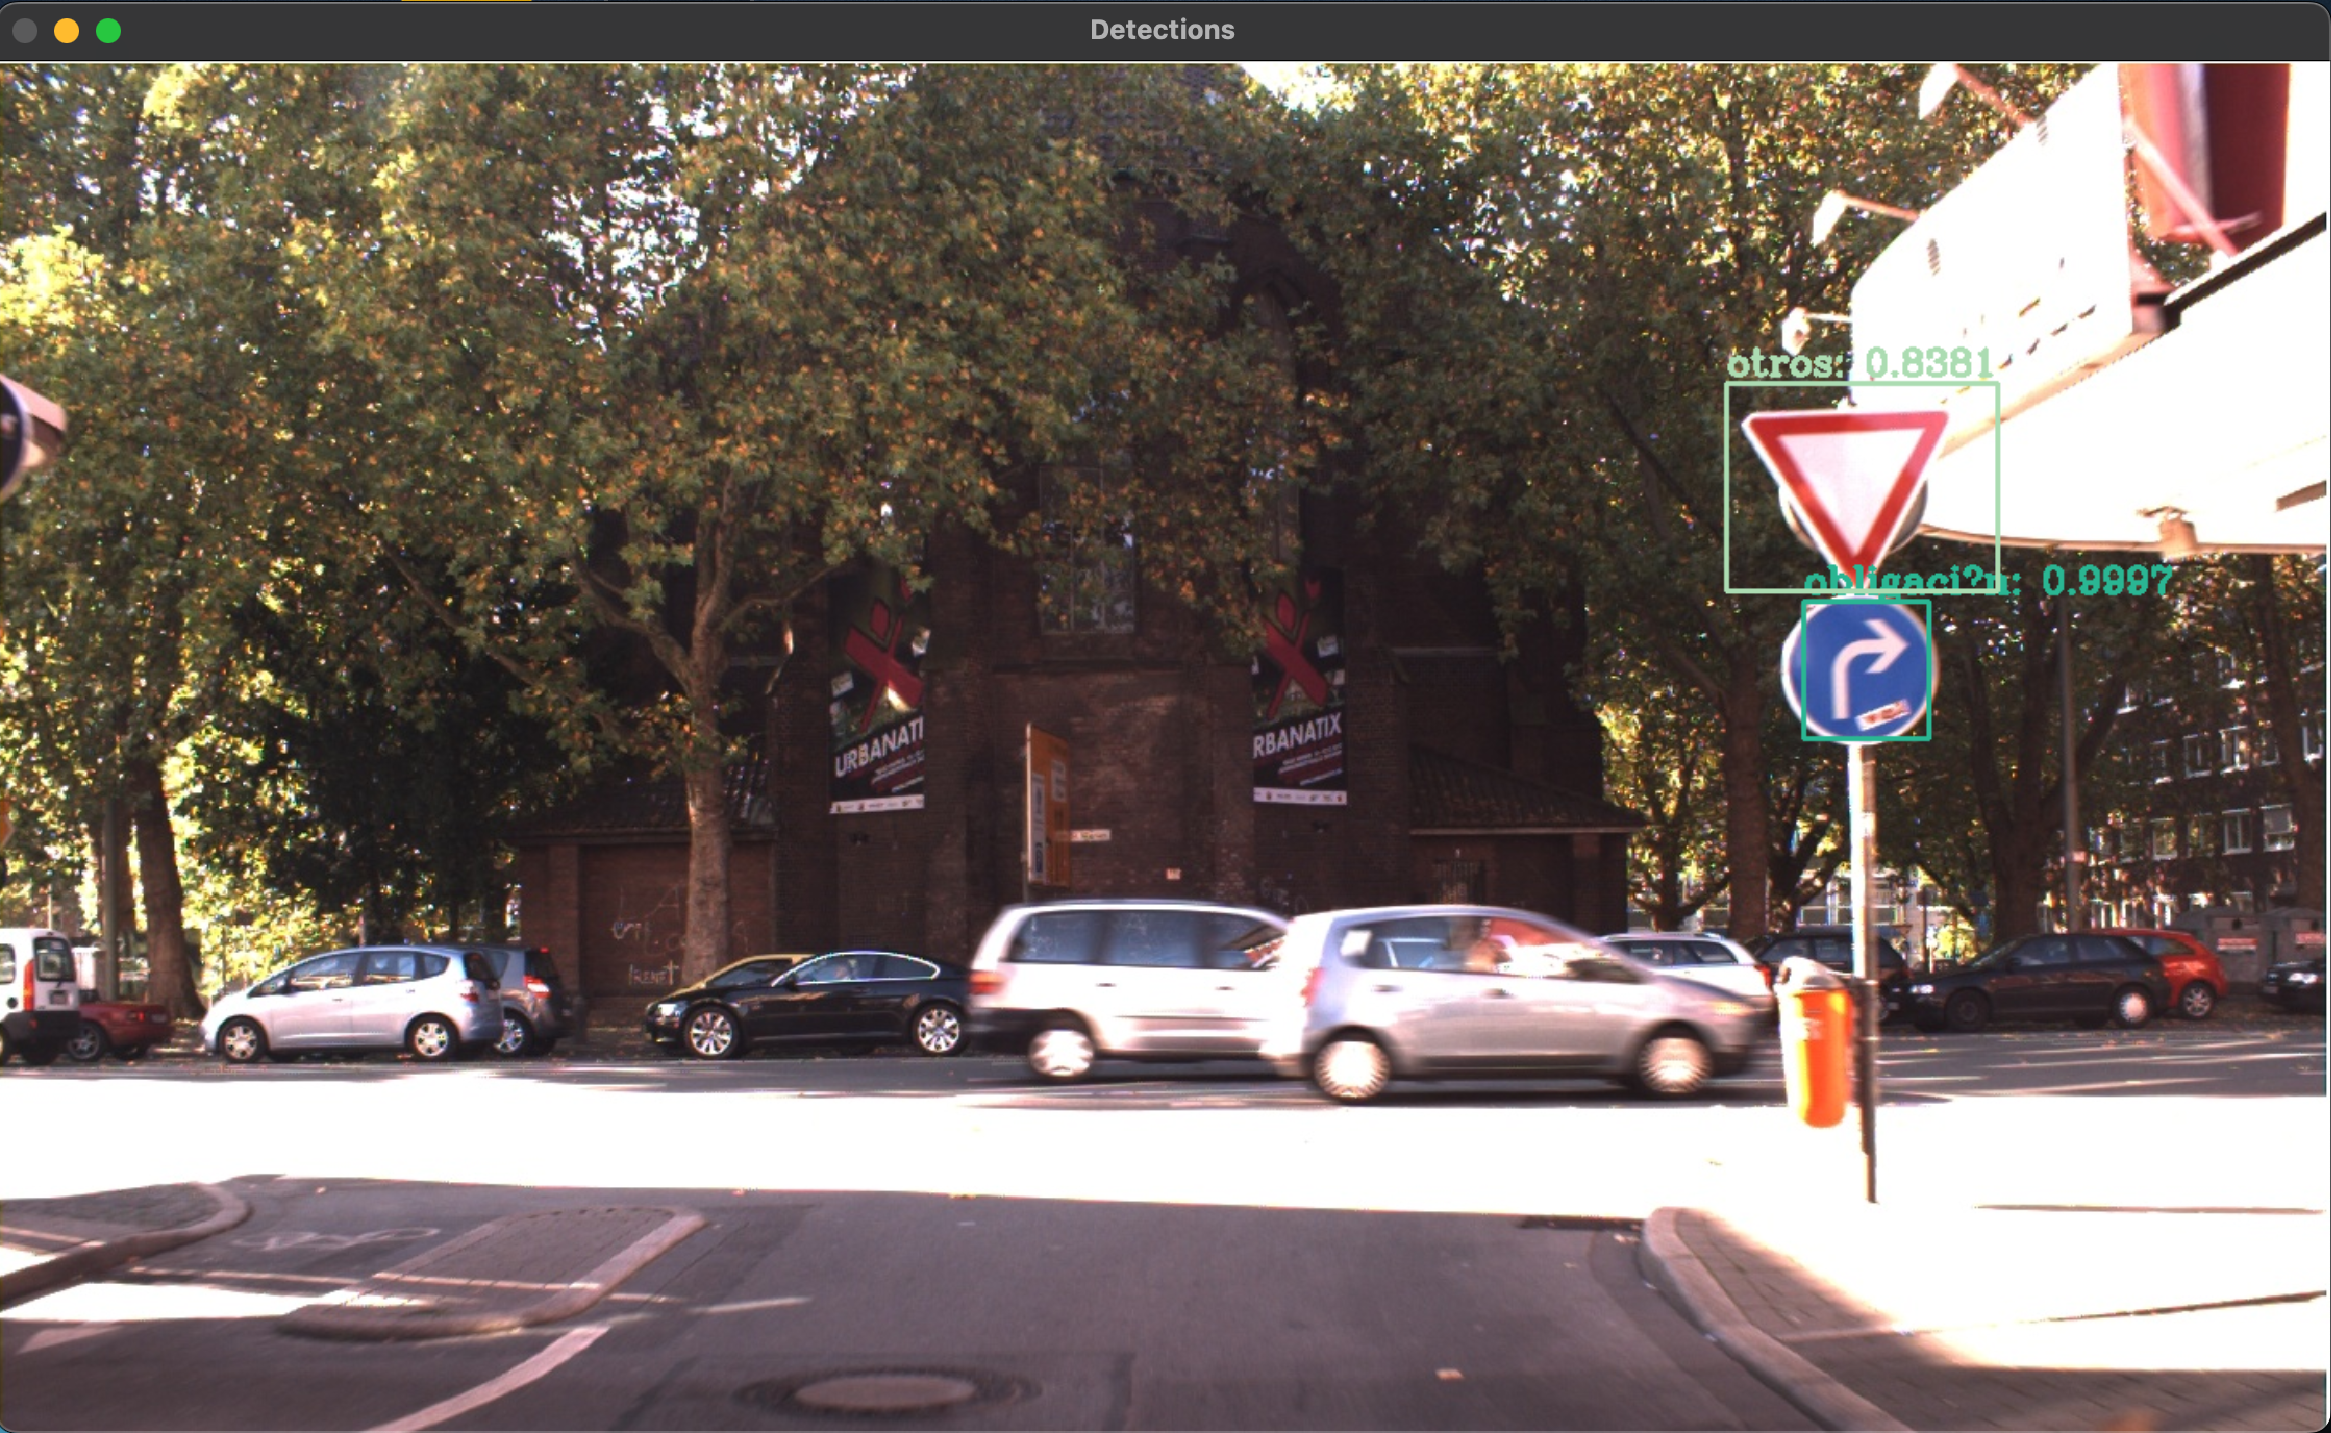
\includegraphics[width=0.6\textwidth]{Imagenes/IA/deteccion1.pdf}
    \caption{Primer ejemplo de detección de señales miniatura en vídeo}
    \label{deteccion1}
\end{figure}

\begin{figure}[H]
    \centering
 	\includegraphics[width=0.6\textwidth]{Imagenes/IA/deteccion2.pdf}
    \caption{Segundo ejemplo de detección de señales miniatura en vídeo}
    \label{deteccion2}
\end{figure}

De igual forma, podemos probar con imágenes de una vía normal, podemos visualizar el procesado de nuestro algoritmo en la figura \ref{deteccion3}\\

\begin{figure}[H]
    \centering
 	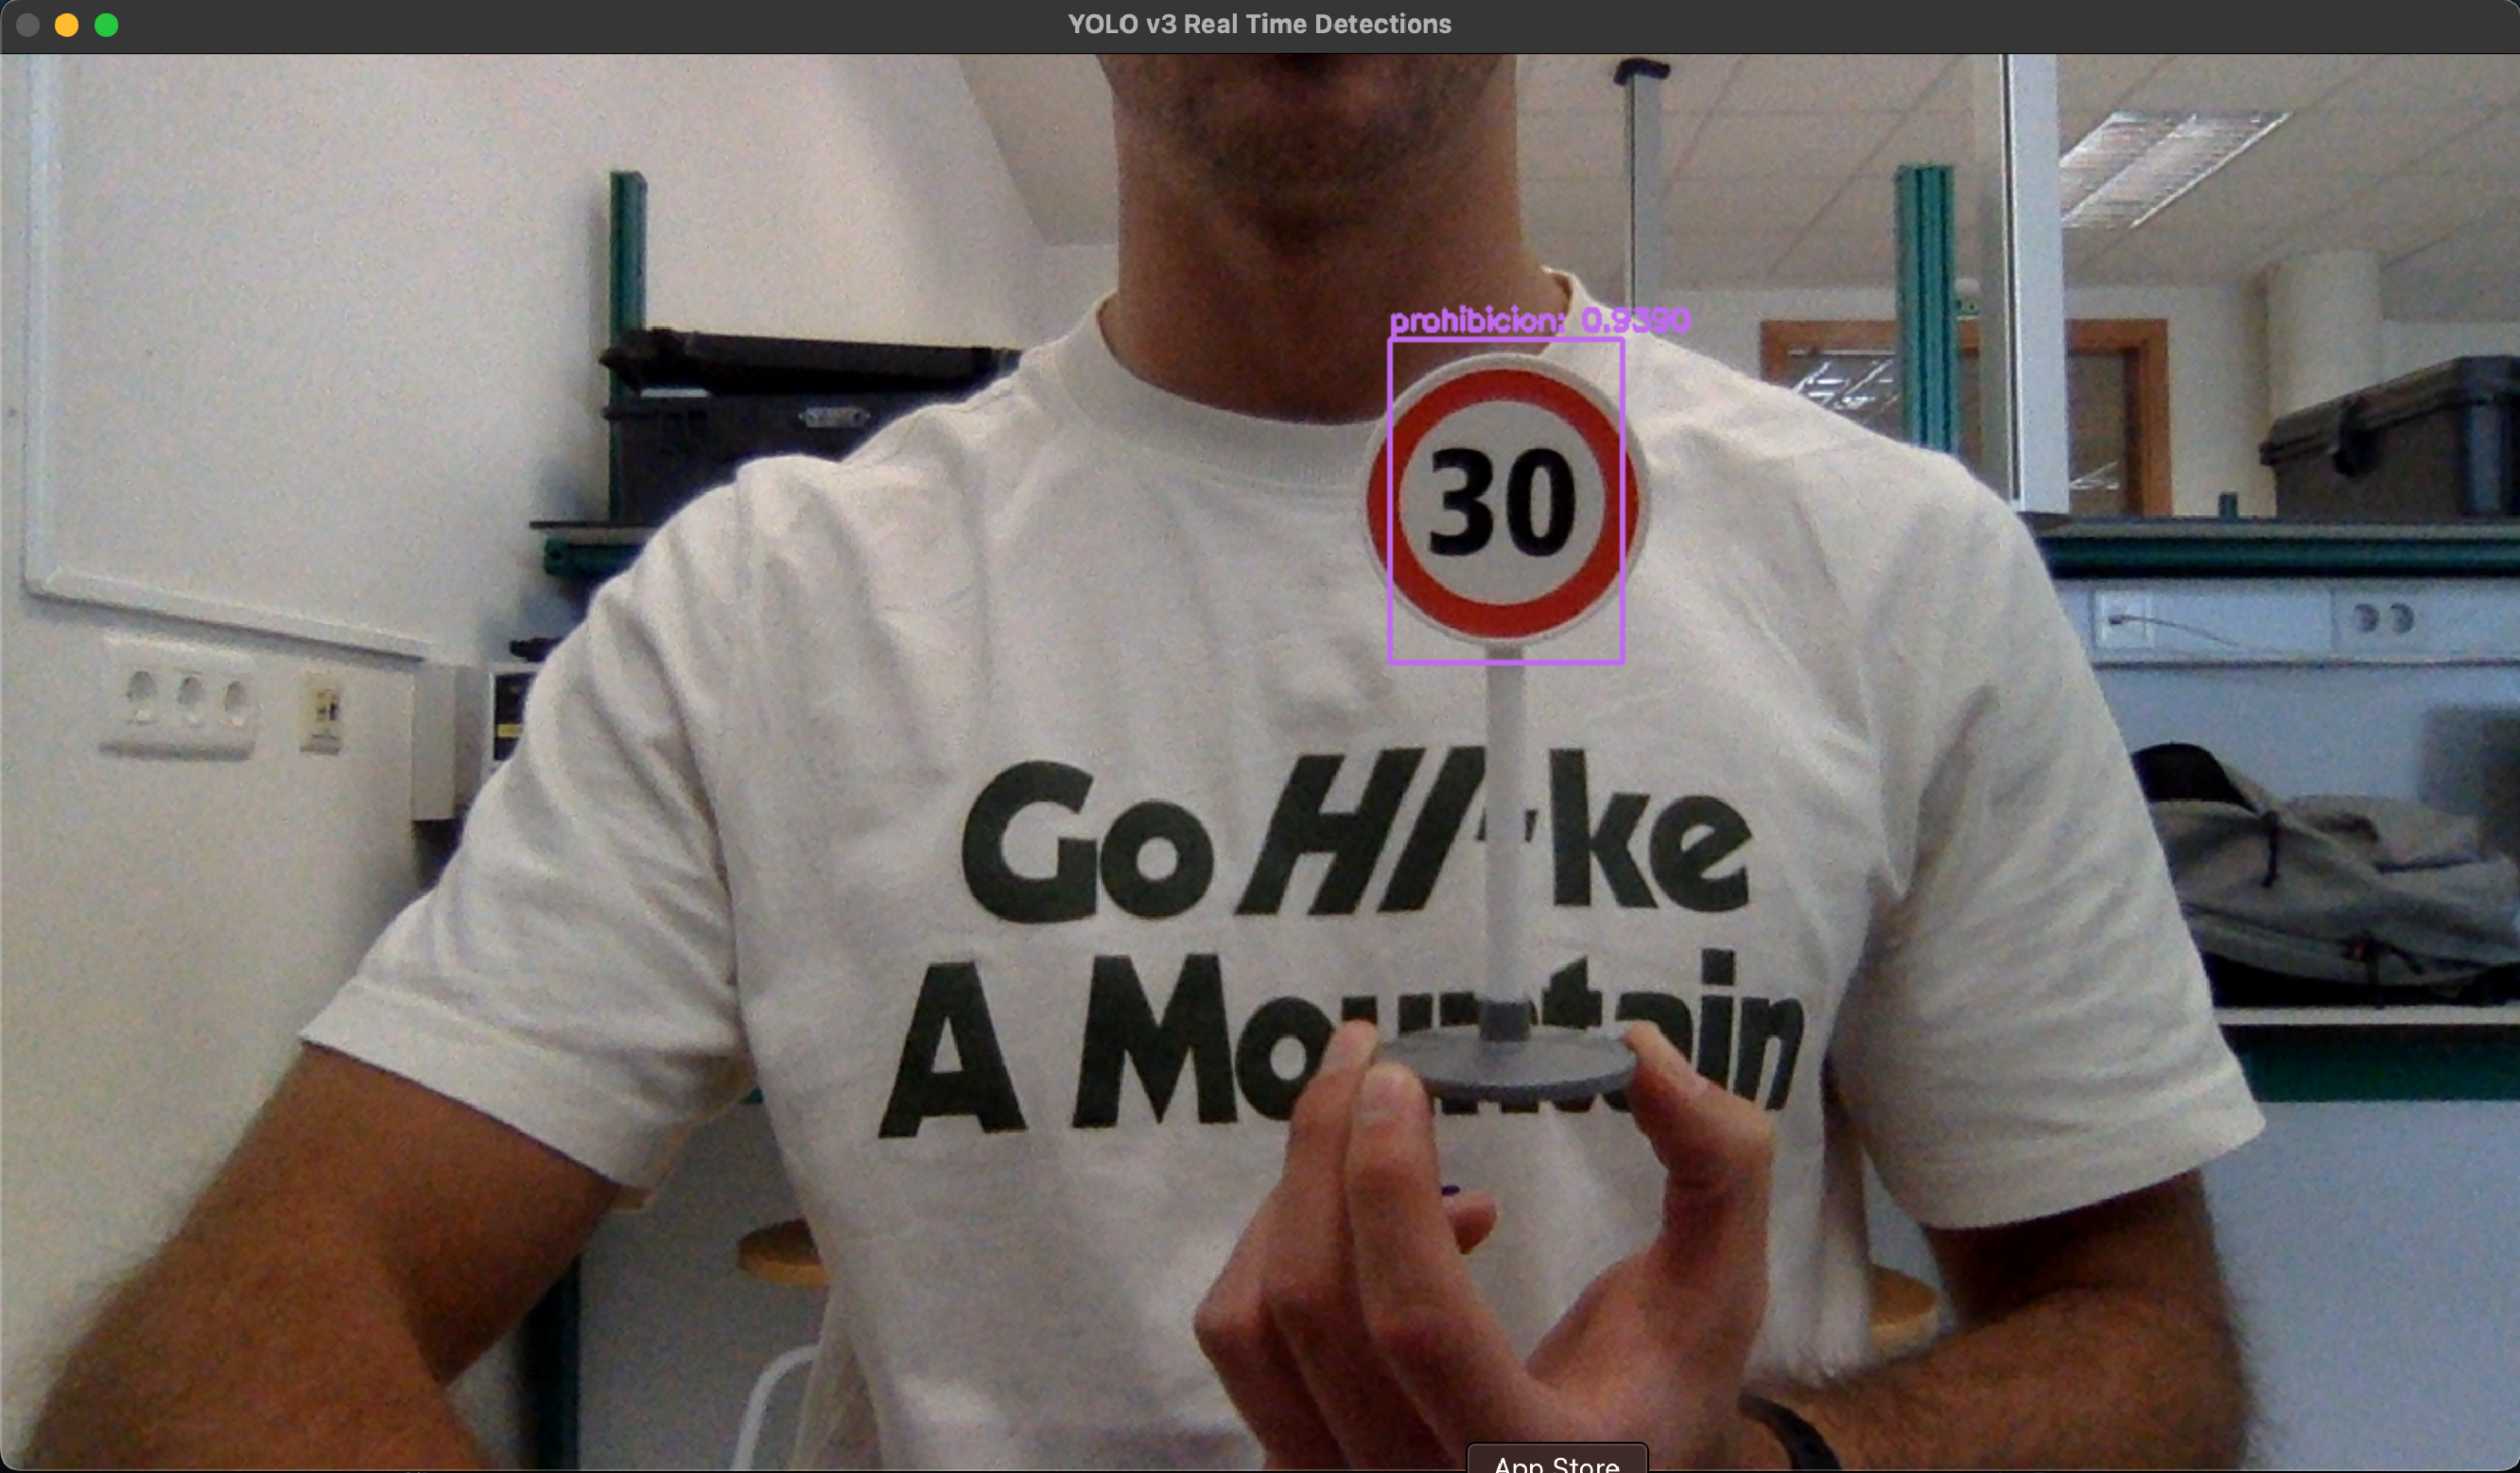
\includegraphics[width=0.6\textwidth]{Imagenes/IA/deteccion3.pdf}
    \caption{Detección de señales reales en vídeo en carretera real}
    \label{deteccion3}
\end{figure}

Finalmente, a través de un popular repositorio de GitHub \url{https://github.com/rafaelpadilla/Object-De\ tection-Metrics.git} dedicado a medir el rendimiento de algoritmos de detección, podremos analizar nuestro sistema de detección de señales. A través de 64 imágenes etiquetadas y procesadas por el algoritmo, podremos medir el rendimiento de la red mediante sus detecciones. En concreto, podremos obtener la curva de Precisión vs Recuperación (Precision vs \textit{Recall}) de nuestro modelo. La precisión es un término que describe la medida verdaderos positivos (TP) en relación con los falsos positivos (FP). Por otro lado, la recuperación se refiere a la proporción de verdaderos positivos (TP) en comparación con la suma de verdaderos positivos y falsos negativos (FN). En resumen, estos conceptos son utilizados para evaluar la efectividad de un modelo de clasificación y se pueden emplear para establecer el límite óptimo del modelo.\\

Para calcular la precisión y la recuperación se hace uso de las siguientes fórmulas:\\
\\
$$\text{precisión} = \frac{\text{TP}}{\text{TP} + \text{FP}}\ \text{recuperación} = \frac{\text{TP}}{\text{TP} + \text{FN}}$$
\\

Podemos contemplar en la figura \ref{rendimiento} que para cada categoría contemplada de señales de tráfico obtenemos una precisión media (AP) diferente. Establecida una probabilidad mínima de detección de 0,5 y threshold de 0,3, para la clase obligación se obtiene una precisión del 57,9\%, para peligro un 72,22\%, para prohibición un 84,54\% y para el resto un 62,14\%. Destacar que entre las 64 imágenes que se han analizado, se encontraban tanto imágenes de señales reales, como señales de juguete, esto es clave porque los pesos pre-entrenados no contaban con señales falsas. Por ello, podemos notar que quizás los valores de precisión obtenidos no son suficientemente altos debido a la inclusión de señales que no se asemejan con las de entrenamiento.\\

\begin{figure}[H]
    \centering
 	\includegraphics[width=\textwidth]{Imagenes/IA/rendimiento.pdf}
    \caption{Gráficas del rendimiento obtenido}
    \label{rendimiento}
\end{figure}

En primer lugar, en conocimiento de que la mayor precisión la hemos obtenido para la clase prohibición con una probabilidad de casi el 85\%, podemos ver que está cerca de parecerse a la curva ideal. La curva ideal que desearíamos sería una curva que se acerque lo máximo posible a la esquina superior derecha, es decir, alta precisión y alto recall. Asimismo, podemos relacionar la curva ideal con el área bajo la curva de precisión, el valor de precisión media obtenido representa el área bajo dicha curva, por lo que si la curva fuese ideal sería claro que el área sería del 100\%.\\

Podemos concluir entonces que la mejor precisión se ha obtenido en la detección de señales de prohibición. Además, destacar el resultado obtenido para la clase peligro, el cual puede llamar la atención por resultar una línea recta en todo momento. Esto se debe a que para todas las imágenes que se han contemplado para medir el rendimiento, el algoritmo ha sido capaz de detectar todas las señales que se han procesado. Este resultado quizás no sea del todo realista, por lo que se podrían añadir un mayor número de imágenes de cada clase para lograr objetivos más fehacientes con la realidad.\\

Una vez montada la estructura principal del sistema de inteligencia artificial, se procedió a intentar implementar nuevas funcionalidades con el objetivo de mejorar las prestaciones. Se decidió entonces dar un paso más allá en la clasificación de las señales, para intentar detectar de qué tipo de señal concreta se trata.\\

Como ya se ha mencionado, entrenar un algoritmo de IA requiere de una capacidad computacional muy alta. Por ello, una forma sencilla de implementar cierta inteligencia que sea capaz de detectar las señales tras procesarlas mediante YOLO, sería la incorporación de una red CNN.\\

Una CNN o Convolutional Neural Network (Red Neuronal Convolucional) es un tipo de arquitectura de red neuronal especialmente diseñada para procesar datos, como imágenes o audio. Ésta destaca por su rendimiento en visión artificial gracias a su capacidad para capturar características locales y patrones espaciales en imágenes, es decir, detección y clasificación de objetos.\\

La consecución de ambas tecnologías, tal y como se ejemplifica en la figura \ref{esquema}, nos permite ciertas ventajas en la consecución de ambas tecnologías:\\

\begin{itemize}
\item 1.	Eficiencia: YOLO destaca por su eficiencia en la detección de objetos, por lo que hacer una detección inicial nos permitirá identificar rápidamente las ubicaciones aproximadas de las señales de tráfico.
\item 2.	Localización precisa: Una vez que YOLO detecta las señales de tráfico, la ubicación de la señal se utiliza para extraer una región más pequeña, que es enviada a las CNN correspondientes para una clasificación más precisa. Al hacer esto, te aseguras de que solo se envíen las regiones relevantes a las CNN, en lugar de toda la imagen, lo que ayuda a mejorar la eficiencia y precisión del proceso de clasificación.
\item 3.	Especialización: Al entrenar las CNN separadas para cada categoría específica de señales de tráfico, logramos una especialización en la clasificación. Como cada CNN se entrena con imágenes específicas, permite una mayor capacidad para aprender características distintivas y patrones asociados a cada tipo de señal.
\end{itemize}

\begin{figure}[H]
    \centering
 	\includegraphics[width=\textwidth]{Imagenes/IA/EsquemaIA.pdf}
    \caption{Ventajas de las diferentes tecnologías}
    \label{esquema}
\end{figure}

El modelo CNN definido consta de varias capas. La estructura de capas que contiene el modelo son las siguientes:\\

\begin{itemize}
\item 1.	Capa de convolución 2D con 16 filtros y tamaño de kernel 3x3, con función de activación ReLU.
\item 2.	Capa de convolución 2D con 32 filtros y tamaño de kernel 3x3, con función de activación ReLU.
\item 3.	Capa de MaxPooling 2D con tamaño de pool 2x2.
\item 4.	Capa de normalización por lotes (Batch Normalization).
\item 5.	Capa de convolución 2D con 64 filtros y tamaño de kernel 3x3, con función de activación ReLU.
\item 6.	Capa de convolución 2D con 128 filtros y tamaño de kernel 3x3, con función de activación ReLU.
\item 7.	Capa de MaxPooling 2D con tamaño de pool 2x2.
\item 8.	Capa de normalización por lotes (Batch Normalization).
\item 9.	Capa de aplanamiento (Flatten).
\item 10.Capa densa (fully connected) con 512 neuronas y función de activación ReLU.
\item 11.Capa de normalización por lotes (Batch Normalization).
\item 12.Capa de Dropout con una tasa de dropout de 0.5.
\item 13.Capa densa (fully connected) con 2 neuronas y función de activación softmax.
\end{itemize}


En total, las CNNs están formadas 13 capas, incluyendo las capas de convolución, capas de pooling, capas de normalización por lotes, capas densas y capas de dropout. Cada una de estas capas realiza las siguientes funciones:\\

\begin{itemize}
\item 1.	Capa de convolución 2D: Realiza la convolución de la imagen de entrada con un conjunto de filtros para extraer características importantes de la imagen. Utiliza una función de activación ReLU para introducir no linealidad en la red.
\item 2.	Capa de convolución 2D: Similar a la capa anterior, realiza otra convolución con un conjunto de filtros diferentes para extraer más características de la imagen. También utiliza la función de activación ReLU.
\item 3.	Capa de MaxPooling 2D: Reduce la dimensión espacial de la salida de las capas anteriores mediante la reducción de la resolución espacial. Ayuda a disminuir la cantidad de parámetros y a aprender características más generales.
\item 4.	Capa de normalización por lotes (Batch Normalization): Normaliza los valores de activación de la capa anterior para acelerar el entrenamiento y mejorar la estabilidad de la red.
\item 5.	Capa de convolución 2D: Realiza otra convolución con más filtros para extraer características más complejas de la imagen.
\item 6.	Capa de convolución 2D: Realiza otra convolución con aún más filtros para capturar características más específicas de la imagen.
\item 7.	Capa de MaxPooling 2D: Reduce la dimensión espacial de la salida de las capas anteriores.
\item 8.	Capa de normalización por lotes (Batch Normalization): Normaliza los valores de activación de la capa anterior.
\item 9.	Capa de aplanamiento (Flatten): Transforma la salida de la capa anterior en un vector unidimensional, preparándola para la entrada a las capas densas.
\item 10.Capa densa (fully connected): Capa de neuronas completamente conectadas donde cada neurona está conectada a todas las neuronas de la capa anterior. Utiliza la función de activación ReLU.
\item 11.Capa de normalización por lotes (Batch Normalization): Normaliza los valores de activación de la capa anterior.
\item 12.Capa de Dropout: Apaga aleatoriamente un porcentaje de las neuronas durante el entrenamiento para evitar el sobreajuste y mejorar la generalización del modelo.
\item 13.Capa densa (fully connected): Capa final de clasificación con 2 neuronas y función de activación softmax. Produce las probabilidades de pertenencia a cada una de las subclases.
\end{itemize}


Fruto del entrenamiento hemos obtenido las matrices de confusión de cada CNN, en una matriz de confusión las filas representan las clases reales y las columnas representan las clases predichas por el modelo, donde cada celda de la matriz muestra la cantidad de ejemplos que pertenecen a una clase específica. La estructura general de este tipo de matrices es la siguiente \ref{genconf} \cite{cm}\\

\begin{figure}[H]
    \centering
 	\includegraphics[width=\textwidth]{Imagenes/IA/general_confusion.pdf}
    \caption{Estructura general de las matrices de confusión}
    \label{genconf}
\end{figure}

Donde el número total de falsos negativos (TFN), falsos positivos (TFP), verdaderos negativos (TTN) y verdaderos positivos son respectivamente (TTP) \ref{forconf}.\\

\begin{figure}[H]
    \centering
 	\includegraphics[width=0.2\textwidth]{Imagenes/IA/formulas_confusion.pdf}
    \caption{Fórmulas de cálculo}
    \label{forconf}
\end{figure}

La categoría peligro se divide en 9 subclases: General caution, Road narrows on the right, Road work, Children crossing, Wild animals crossing, Caution roundabout, Caution traffic light, Caution planes y 10\% slope. En su matriz de confusión, encontrada en la figura \ref{pelconf}, detectamos que no se ha producido ninguna detección falsa y que el número de verdaderos positivos es elevado, es decir, el modelo entrenado para las clases de peligro está teniendo un rendimiento muy bueno en términos de clasificación.\\

\begin{figure}[H]
    \centering
 	\includegraphics[width=\textwidth]{Imagenes/IA/peligro_confusion.pdf}
    \caption{Matriz de confusión para la categoría peligro}
    \label{pelconf}
\end{figure}

La categoría obligación se divide en 3 subclases: Mandatory straight, Mandatory right y Mandatory left. En la figura \ref{obconf} podemos ver su matriz de confusión, los resultados son análogos a los observados en las clases comentadas para la categoría peligro.\\

\begin{figure}[H]
    \centering
 	\includegraphics[width=\textwidth]{Imagenes/IA/obligacion_confusion.pdf}
    \caption{Matriz de confusión para la categoría obligación}
    \label{obconf}
\end{figure}

La tercera de las clases que tenemos tras la detección en YOLO es prohibición, que se divide en 6 subclases: No passing, Speed limit (30km/h), Speed limit (90km/h), Priority in opposite direction, No overtaking, Horn prohibited. Analizando los resultados de la figura \ref{probconf} nos damos cuenta de que por primera vez nos encontramos detecciones falsas, sin embargo, la cifra es anecdótica comparada con las detecciones verdaderas.\\

\begin{figure}[H]
    \centering
 	\includegraphics[width=\textwidth]{Imagenes/IA/prohibicion_confusion.pdf}
    \caption{Matriz de confusión para la categoría prohibición.}
    \label{probconf}
\end{figure}

Finalmente, la última clase otros se divide en 2 subclases: No passing y Stop y los resultados son equivalentes a los tres anteriores \ref{otrosconf}.\\

\begin{figure}[H]
    \centering
 	\includegraphics[width=\textwidth]{Imagenes/IA/otros_confusion.pdf}
    \caption{Matriz de confusión para la útltima categoría.}
    \label{otrosconf}
\end{figure}


Llevando a la práctica la incorporación de las redes CNN veremos realmente si son fiables, por ello, procederemos a ver cómo se desenvuelve en el propio vehículo de Amazon. Montando una prueba con el coche y varías señales nos encontramos con los siguientes resultados \ref{c1}, \ref{c2}, \ref{c3}, \ref{c4}.\\

\begin{figure}[H]
    \centering
 	\includegraphics[width=\textwidth]{Imagenes/IA/YoloCNN_coche.pdf}
    \caption{Resultados de la prueba (1).}
    \label{c1}
\end{figure}


\begin{figure}[H]
    \centering
 	\includegraphics[width=\textwidth]{Imagenes/IA/YoloCNN_coche2.pdf}
    \caption{Resultados de la prueba (2).}
    \label{c2}
\end{figure}

\begin{figure}[H]
    \centering
 	\includegraphics[width=\textwidth]{Imagenes/IA/YoloCNN_coche3.pdf}
    \caption{Resultados de la prueba (3).}
    \label{c3}
\end{figure}

\begin{figure}[H]
    \centering
 	\includegraphics[width=\textwidth]{Imagenes/IA/YoloCNN_coche3.pdf}
    \caption{Resultados de la prueba (4).}
    \label{c4}
\end{figure}

Sin embargo, a pesar de quedar satisfechos con los resultados obtenidos, hemos encontrado ocasiones en las que no detecta bien cada señal, como podemos observar en la señal de limitación 30 km/h \ref{fallo}. \\

\begin{figure}[H]
    \centering
 	\includegraphics[width=\textwidth]{Imagenes/IA/ejemplo_fallo.pdf}
    \caption{Fallo de detección.}
    \label{fallo}
\end{figure}

Esto puede ser debido a que las condiciones de calidad de imagen que se obtienen de la cámara del propio vehículo no son exactamente las mismas que las imágenes con las que ha sido entrenado. De cara a líneas futuras sería interesante que el conjunto de imágenes creado para el entrenamiento, se diseñara a partir de vídeos grabados por coche.\\

En último lugar, según se puede constatar en el Anexo I apartado 6.2, también hemos utilizado una herramienta de etiquetado denominada LabelIMG \url{https://github.com/heartexlabs/labelImg}. Sería recomendable atender al manual de desarrollador incluido en el Anexo I para aprender a manejar o conocer más detalles acerca del sistema de inteligencia artificial.




	\section{Normativa}

\chapter{Costes}

\chapter{Rendimiento: Validación del servicio}

\chapter{Anexo I: Manual del desarrollador}
	\section{Software}	

	\section{Componentes}

	\section{Infraestructura de la red}
		En el proceso de creación de la red 4G, se siguieron los siguientes pasos:

\begin{enumerate}
\item Descarga de la última versión de \textbf{Ubuntu}, \textbf{22.04 LTS}.
\item Grabación de la ISO en un pincho a través de \textbf{UNetbootin} y posterior instalación de Linux en el ordenador.
\item Instalación de los drivers de la \textit{Blade} siguiendo el manual de \textit{GitHub}:\\
 \url{https://github.com/Nuand/bladeRF/wiki/Getting-Started:-Linux}

\begin{lstlisting}
sudo add-apt-repository ppa:nuandllc/bladerf
sudo apt-get update
sudo apt-get install bladerf
\end{lstlisting}

\item Instalación de \textbf{srsran} siguiendo el manual de GitHub y las librerías \textbf{boost} y \textbf{libboost}:\\
\url{https://docs.srsran.com/projects/4g/en/latest/general/source/1_installation.html}\\
\url{https://docs.srsran.com/projects/4g/en/latest/getting_started.html}

\begin{lstlisting}
git clone https://github.com/srsRAN/srsRAN_4G.git
cd srsRAN_4G
mkdir build
cd build
cmake ../
make
make test
sudo make install
srsran_4g_install_configs.sh user
\end{lstlisting}

\item Modificación de los archivos de configuración que se encuentran en la ruta \textit{root/.config/srsran/}:
\begin{itemize}
	\item epc.conf
	\item enb.conf
	\item user_db.csv
\end{itemize}

En el archivo \textbf{enb.conf} se cambiaron los valores de \textbf{MCC} y \textbf{MNC} que están disponibles en la SIM, y se establecieron los valores correspondientes al \textbf{MCC} y \textbf{MNC} utilizados en el proyecto (\textbf{901-70}) para que se correspondan con el IMSI de las SIM. También se modificó el \textbf{dl_earfcn} utilizando una página web y se estableció el ancho de banda \textbf{n_prb} en \textbf{50}.\\

En el archivo \textbf{epc.conf} se modificaron los valores de \textbf{MCC} y \textbf{MNC} y se añadieron los nombres de la red con:
\begin{lstlisting}
    full_net_name= NOMBRE
    short_net_name= NOMBRE
\end{lstlisting}

En el archivo \textbf{user_db.csv} se creó un usuario nuevo con la siguiente información:
\begin{lstlisting}
    nombre, mil (Auth), IMSI (aparece en las hojas de las sims),
    KEY (aparece en las hojas de las sims), opc,
    OPC(aparece en las hojas de las sims), 9000,
    sqn (se pone automáticamente, pero pon números, por ejemplo todo a 0),
    7 (QCI), dynamic (IP_alloc)
\end{lstlisting}

\item Para crear la red y que funcione, se siguieron los siguientes pasos:
\begin{lstlisting}
    srepc_if_masq.sh enp0s25
    srsepc epc.conf
    srsenb enb.conf
\end{lstlisting}

\item Una vez obtenida la conexión a internet con la red 4G, nos bajamos los ficheros \textit{python} de control del coche para crear el servidor cloud e instalamos el servidor \textbf{MQTT Mosquitto}.

\item Modificamos el fichero de configuración /etc/mosquitto/mosquitto.conf con las siguientes líneas:
\begin{lstlisting}
	persistence true
	persistence_location /var/lib/mosquitto/
	allow_anonymous true
	listener 1883 10.0.128.176
	bind_interface enp0s25
	log_type information
	log_type warning
	log_type error
\end{lstlisting}

\item Para el correcto funcionamiento del servidor \textbf{MQTT Mosquitto} hay que suscribirse a los tópicos cada vez que lo ejecutamos con el siguiente comando:
\begin{lstlisting}
	mosquitto_sub -h localhost -t 1\#
\end{lstlisting}


\item Para el correcto funcionamiento del servidor \textbf{MQTT Mosquitto} hay que suscribirse a los tópicos cada vez que lo ejecutamos con el siguiente comando:
\begin{lstlisting}
	mosquitto_sub -h localhost -t 1\#
\end{lstlisting}

\item Por otra parte, en el dispositivo utilizado como cliente \textbf{MQTT Mosquitto} hay que suscribirse a los diferentes tópicos del vehículo, mostrando uno como ejemplo:
\begin{lstlisting}
	1/AM-Cloud
\end{lstlisting}
Y, publicarlos:
\begin{lstlisting}
	Topic: 1/command
	Message: AM-Cloud
\end{lstlisting}


\item Por último, para lanzar el servicio \textbf{MQTT Mosquitto} y otras acciones como relanzarlo, ver su estado o pararlo utilizamos los siguientes comandos:
\begin{lstlisting}
	sudo systemctl start mosquitto
	sudo systemctl status mosquitto
	sudo systemctl restart mosquitto
	sudo systemctl stop mosquitto
\end{lstlisting}

\end{enumerate}
	
	\section{Modelos de IA}	

	\section{Identificación de imágenes}
	
\chapter{Anexo II: Planificación}

\chapter{Referencias}

\end{document}